\documentclass[12pt]{article}
\usepackage{graphicx}
\usepackage{hyperref}
\usepackage[top=2.75in, left=1in, right=1in, bottom=0.25in]{geometry}
\usepackage[utf8]{inputenc}
\usepackage[english]{babel}
\usepackage{fancyhdr}
\usepackage[utf8]{inputenc}
\usepackage{listings}
\usepackage{color}
\usepackage[final]{pdfpages}
\usepackage{multirow}
\usepackage{array}
\usepackage{caption}
\usepackage{subcaption}


\definecolor{codegreen}{rgb}{0,0.6,0}
\definecolor{codegray}{rgb}{0.5,0.5,0.5}
\definecolor{codepurple}{rgb}{0.58,0,0.82}
\definecolor{backcolour}{rgb}{0.95,0.95,0.92} 
\lstdefinestyle{mystyle}{
    backgroundcolor=\color{backcolour},   
    commentstyle=\color{codegreen},
    keywordstyle=\color{magenta},
    numberstyle=\tiny\color{codegray},
    stringstyle=\color{codepurple},
    basicstyle=\footnotesize,
    breakatwhitespace=false,         
    breaklines=true,                 
    captionpos=b,                    
    keepspaces=true,                 
    numbers=left,                    
    numbersep=5pt,                  
    showspaces=false,                
    showstringspaces=false,
    showtabs=false,                  
    tabsize=2
} 
\lstset{style=mystyle}

\setlength{\parindent}{4em}
\setlength{\parskip}{1em}
\pagestyle{fancy}
\fancyhf{}
\rhead{Assignment 5}
\lhead{Huan Huang}
\renewcommand{\headrulewidth}{0.4pt}
\renewcommand{\footrulewidth}{0.4pt}
\rfoot{Page \thepage}


\begin{document}
\begin{titlepage}
	\begin{center}
	\Huge{Web Science cs532-s16}\\
	[0.25in]
	\textsc{\Large Assignment 5 Report}\\
	\textsc{\normalsize Dr. Michael L. Nelson}\\
	[4.25in]
	\textsc{\normalsize By: Huan Huang}\\
	\large 03/03/2016\\
	
	
	\end{center}
\end{titlepage}
\newpage

\newgeometry{margin=1in}

\section*{Problem 1}

We know the result of the Karate Club (Zachary, 1977) split.
Prove or disprove that the result of split could have been predicted
by the weighted graph of social interactions.  How well does the
mathematical model represent reality?

Generously document your answer with all supporting equations, code,
graphs, arguments, etc.

\noindent
Useful sources include:

\noindent
* Original paper

\noindent
http://aris.ss.uci.edu/~lin/76.pdf

\noindent
* Slides

\begin{verbatim}
http://www-personal.umich.edu/~ladamic/courses/networks/si614w06/ppt/lecture18.ppt

\noindent
http://clair.si.umich.edu/si767/papers/Week03/Community/CommunityDetection.pptx
\end{verbatim}

\noindent
* Code and data

\begin{verbatim}
http://networkx.github.io/documentation/latest/examples/graph/karate_club.html

http://nbviewer.ipython.org/url/courses.cit.cornell.edu/info6010/resources/11notes.ipynb

http://stackoverflow.com/questions/9471906/what-are-the-differences-between-community-detection-algorithms-in-igraph/9478989#9478989

http://stackoverflow.com/questions/5822265/are-there-implementations-of-algorithms-for-community-detection-in-graphs

http://konect.uni-koblenz.de/networks/ucidata-zachary

http://vlado.fmf.uni-lj.si/pub/networks/data/ucinet/ucidata.htm#zachary

https://snap.stanford.edu/snappy/doc/reference/CommunityGirvanNewman.html

http://igraph.org/python/doc/igraph-pysrc.html#Graph.community_edge_betweenness
\end{verbatim}


\subsection*{Answer}
It is very easy to solve this problem, so long you can find the right data source and tools. I found my data from a Nexus web page \url{http://nexus.igraph.org/api/dataset_info?id=1&format=html}. This page provides well designed plot-able files which contain the members of the club(name), connections(edges), weight of the edges, groups the members belong to after the split(factions). All the data and relations in these files are based on Zachery's study of the Karate Club. 

\begin{figure}[h]
\centering
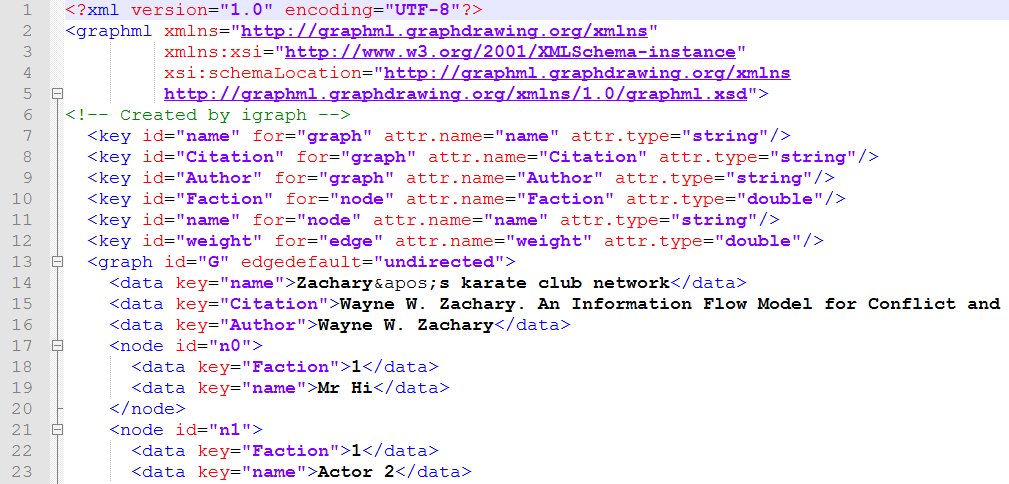
\includegraphics[width=6.5in]{Graphml.png}
\caption{Sample of the data file karate.GraphMl}
\end{figure}

Now, I have the right data source, I just have to use the right tool to plot it. The plotting module I decided to use is python-igraph. It is designed to handle jobs like this problem. To plot the graph, load the data, decide the layout, and set the options in the actual plotting command. For all of the graphs in problem 1, I used circular layout, I found it easier to do comparison with circular layout. Since we are looking for the relationships of the club members, the ``name" is use to set as vertexes, and each vertex is label with the attribute of corresponding ``name" key. Here are the sources where I learned how to use python-igraph: \url{http://igraph.org/python/doc/tutorial/tutorial.html}, \href{http://stackoverflow.com/questions/25254151/using-igraph-in-python-for-community-detection-and-writing-community-number-for}{A Stackoverflow page}, \url{http://igraph.org/python/doc/igraph.Graph-class.html}.

Next, I have to identify the groups after the split. Since the data file already given each individual the faction they split into, therefore, I can identify the two groups by giving the members different colors based on their faction number. Faction 1 is red, faction 2 is blue.
\newpage

\begin{figure}[h]
\centering
\begin{minipage}{.5\textwidth}
  \centering
  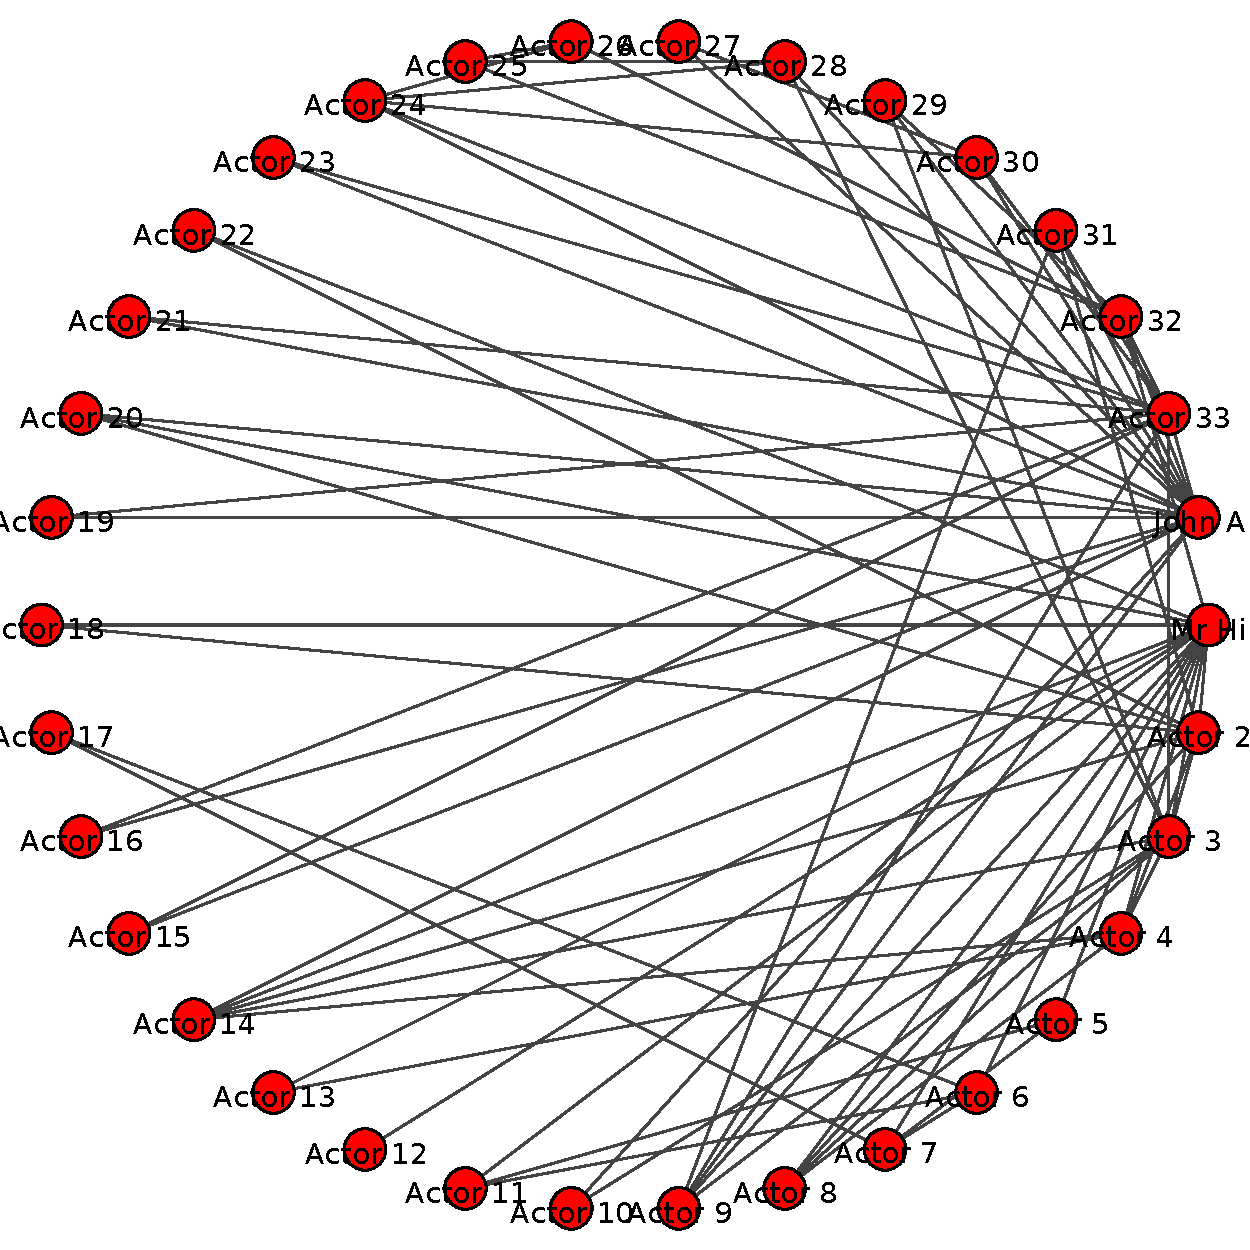
\includegraphics[width=2.5in]{beforesplit.pdf}
  \captionof{figure}{Karate Club before the split}
\end{minipage}%
\begin{minipage}{.5\textwidth}
  \centering
  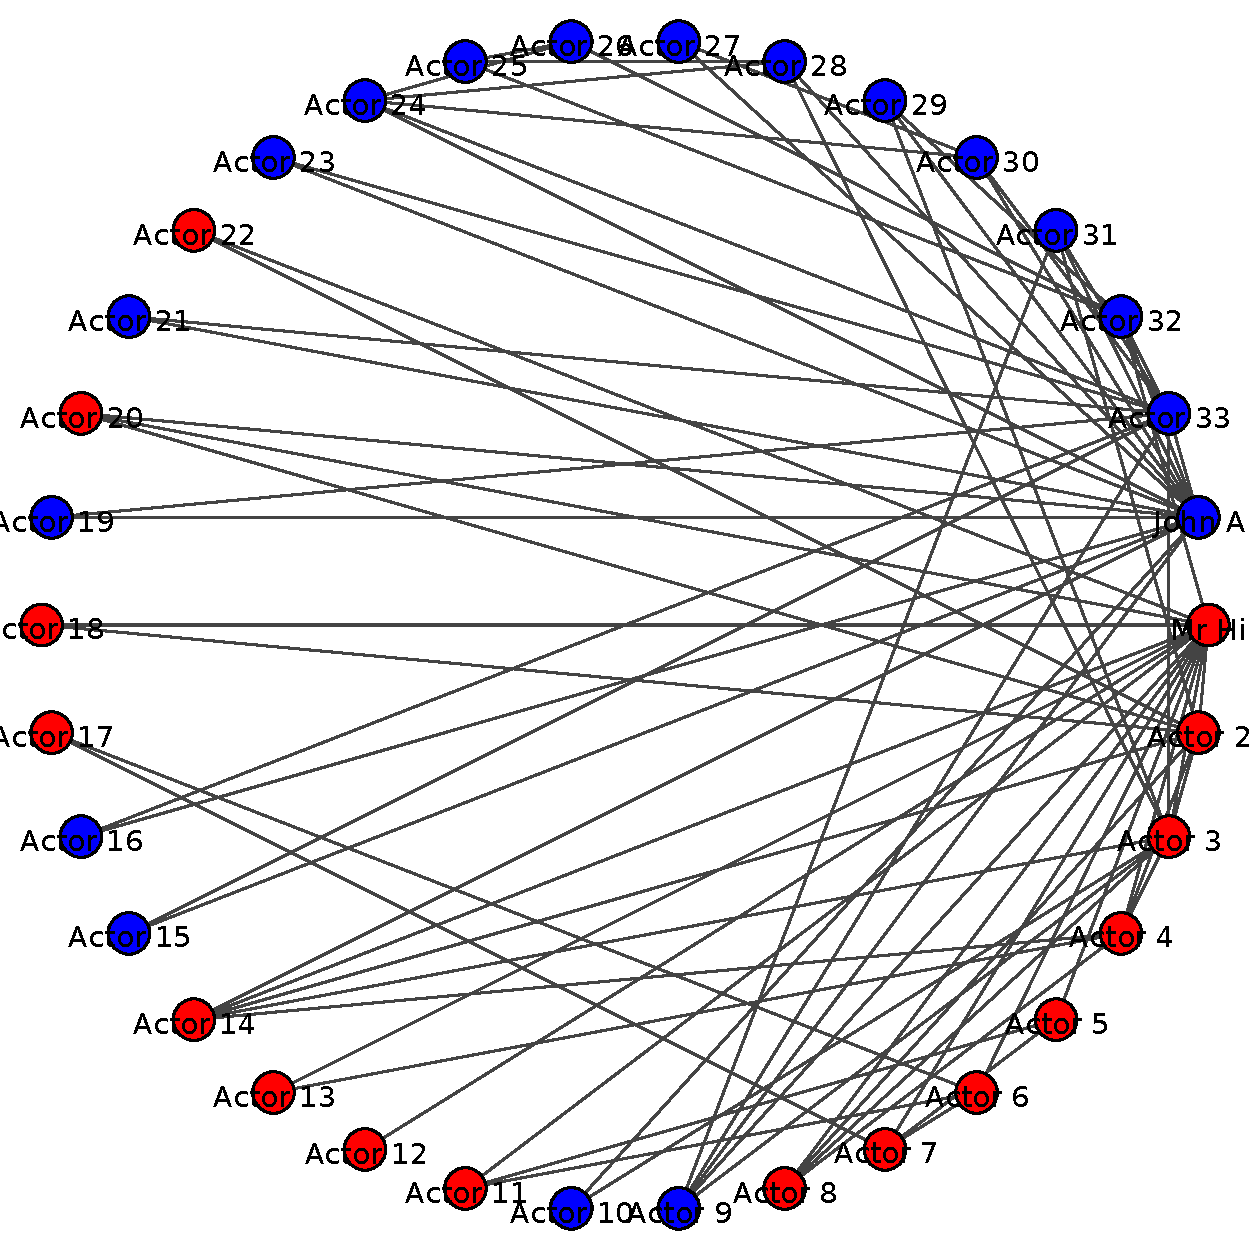
\includegraphics[width=2.5in]{aftersplit.pdf}
  \captionof{figure}{Karate club after the split}
\end{minipage}
\end{figure}

The graphs above shows the actual separation of the karate club which is according to Zachery's study. For the next part of this assignment, I will use community detection algorithms to predict the outcome of the split based on the edges and weight of the edges. 

Of all the community detection algorithms in python-igraph, Girvan Newman's Edgebetweenness and Leading Eigenvectors are the only 2 algorithms that let me decide how many groups the members split into by setting the cluster number. There, I decide to try both of them. 

\begin{figure}[h]
\centering
\begin{minipage}{.5\textwidth}
  \centering
  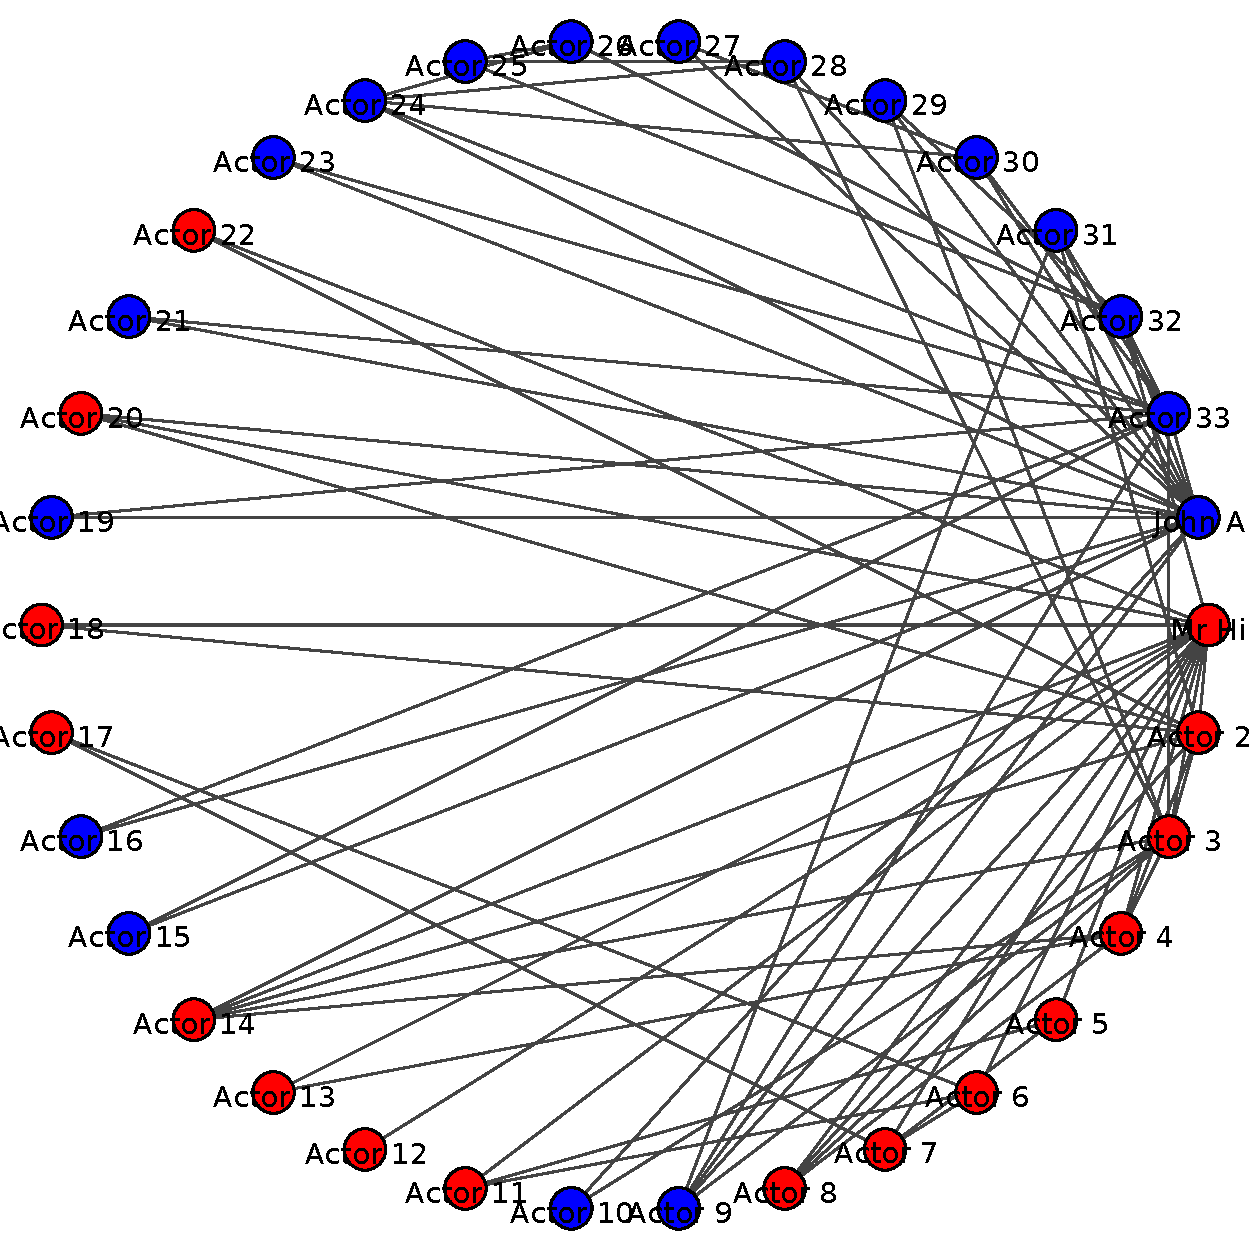
\includegraphics[width=2.5in]{aftersplit.pdf}
  \captionof{figure}{The actual split}
\end{minipage}%
\begin{minipage}{.5\textwidth}
  \centering
  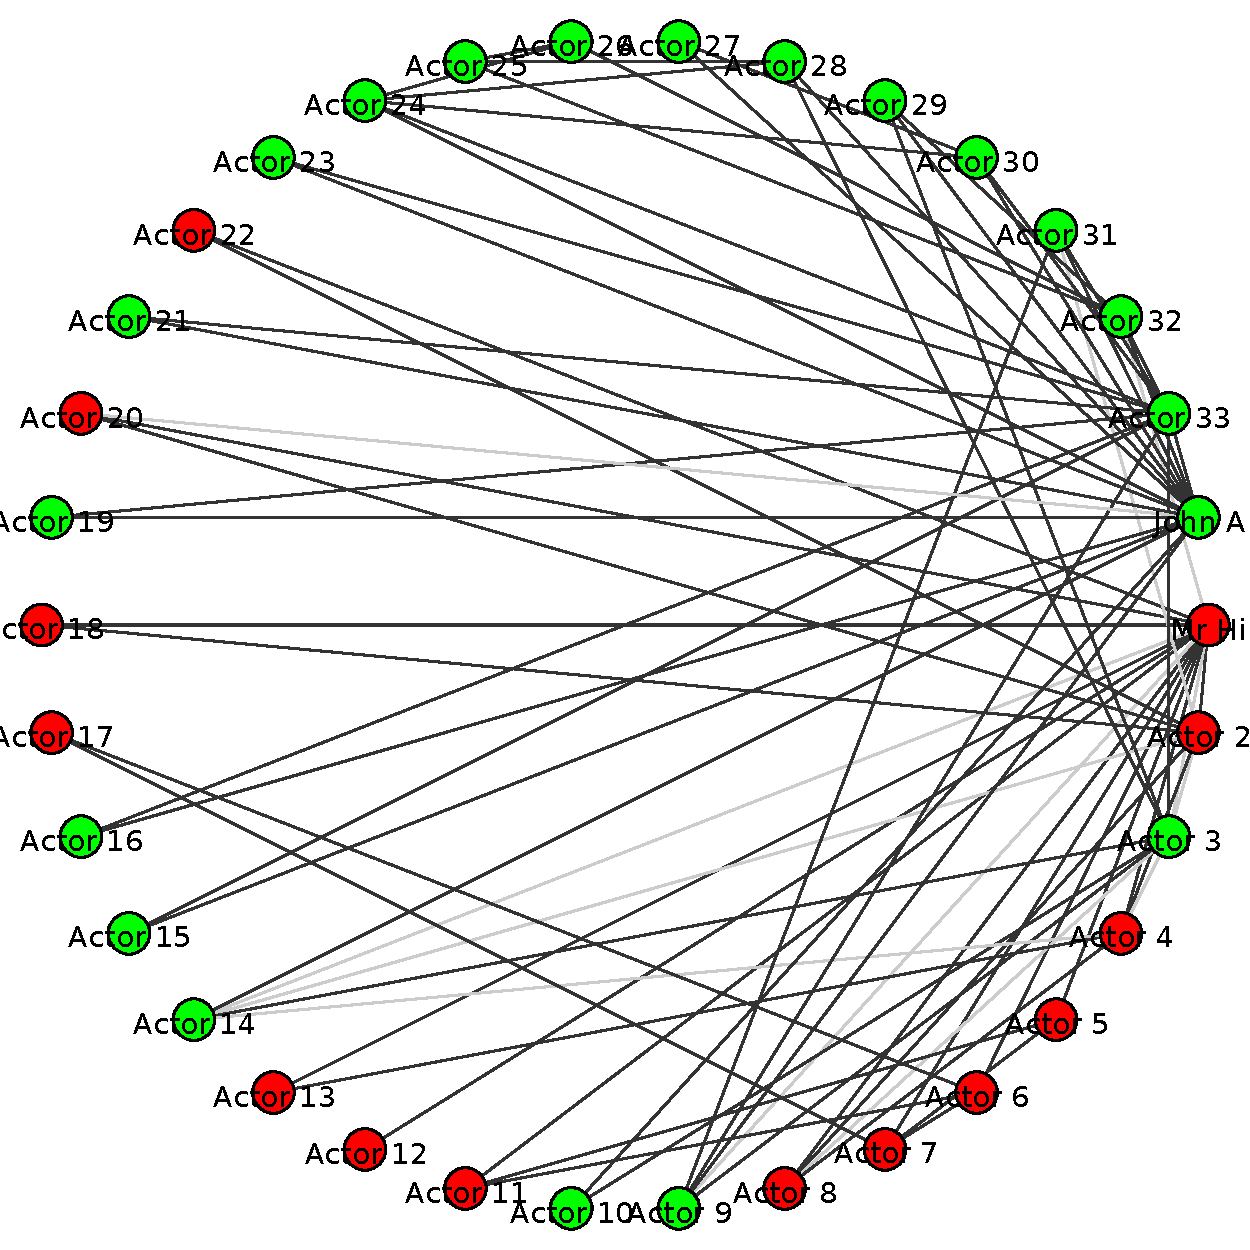
\includegraphics[width=2.5in]{betweenness2.pdf}
  \captionof{figure}{Prediction of Edgebetweenness}
\end{minipage}
\end{figure}

Newman's Edgebetweenness did a pretty good job of predicting the split. It got almost every thing right except actor 3 and 14.
\newpage

\begin{figure}[h]
\centering
\begin{minipage}{.5\textwidth}
  \centering
  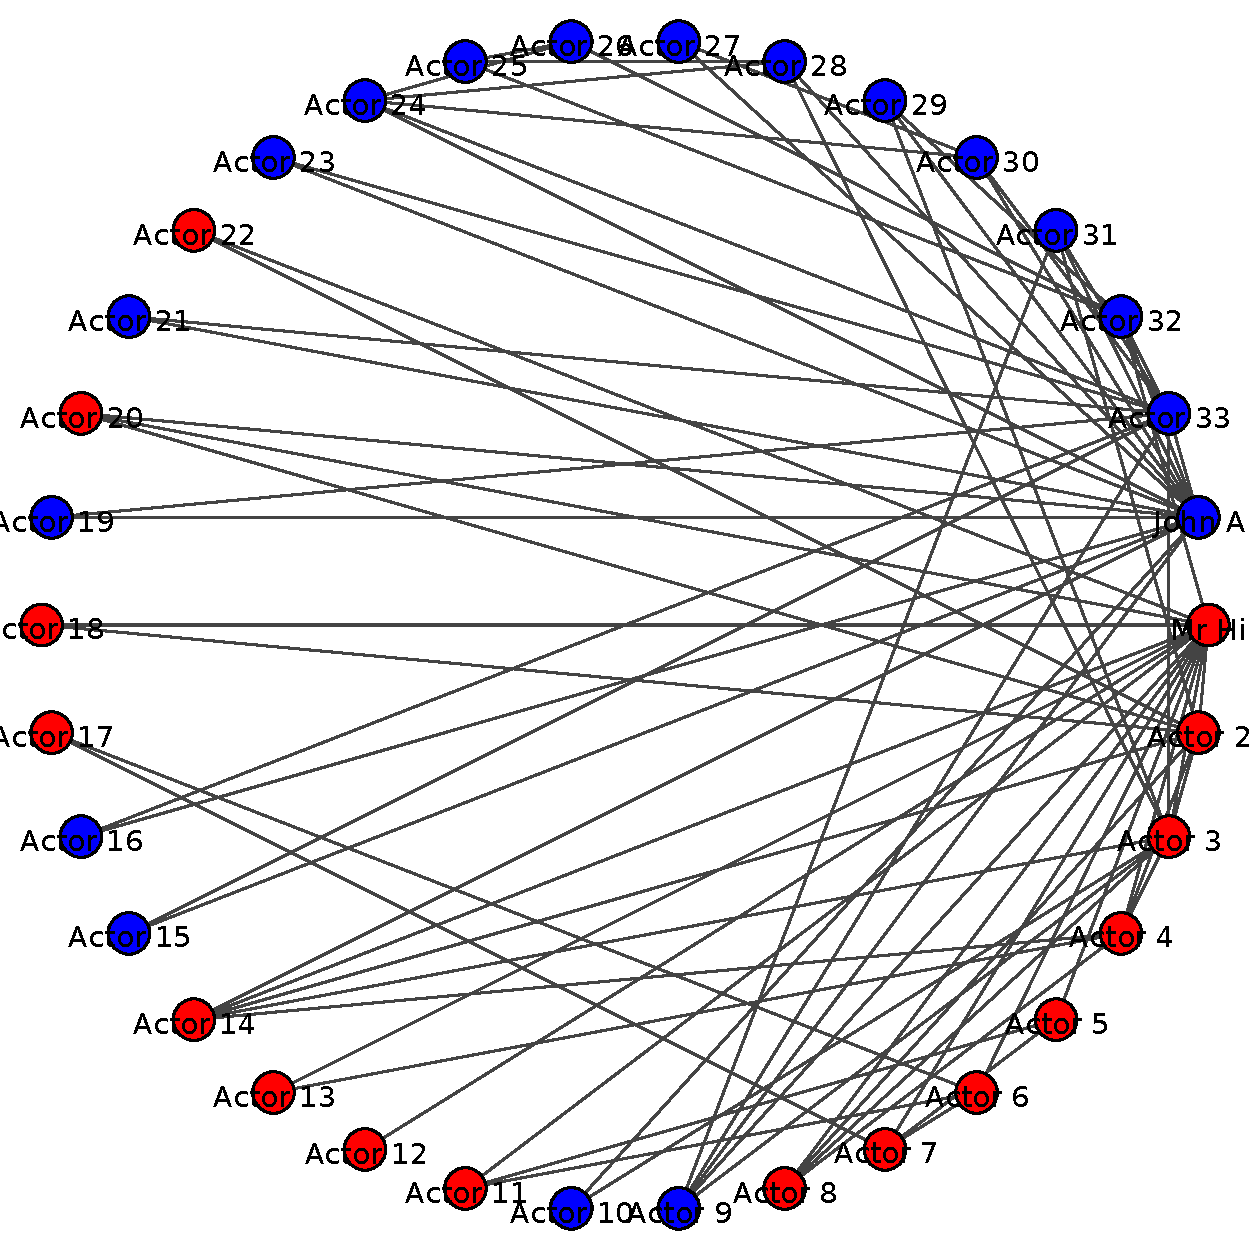
\includegraphics[width=2.5in]{aftersplit.pdf}
  \captionof{figure}{The actual split}
\end{minipage}%
\begin{minipage}{.5\textwidth}
  \centering
  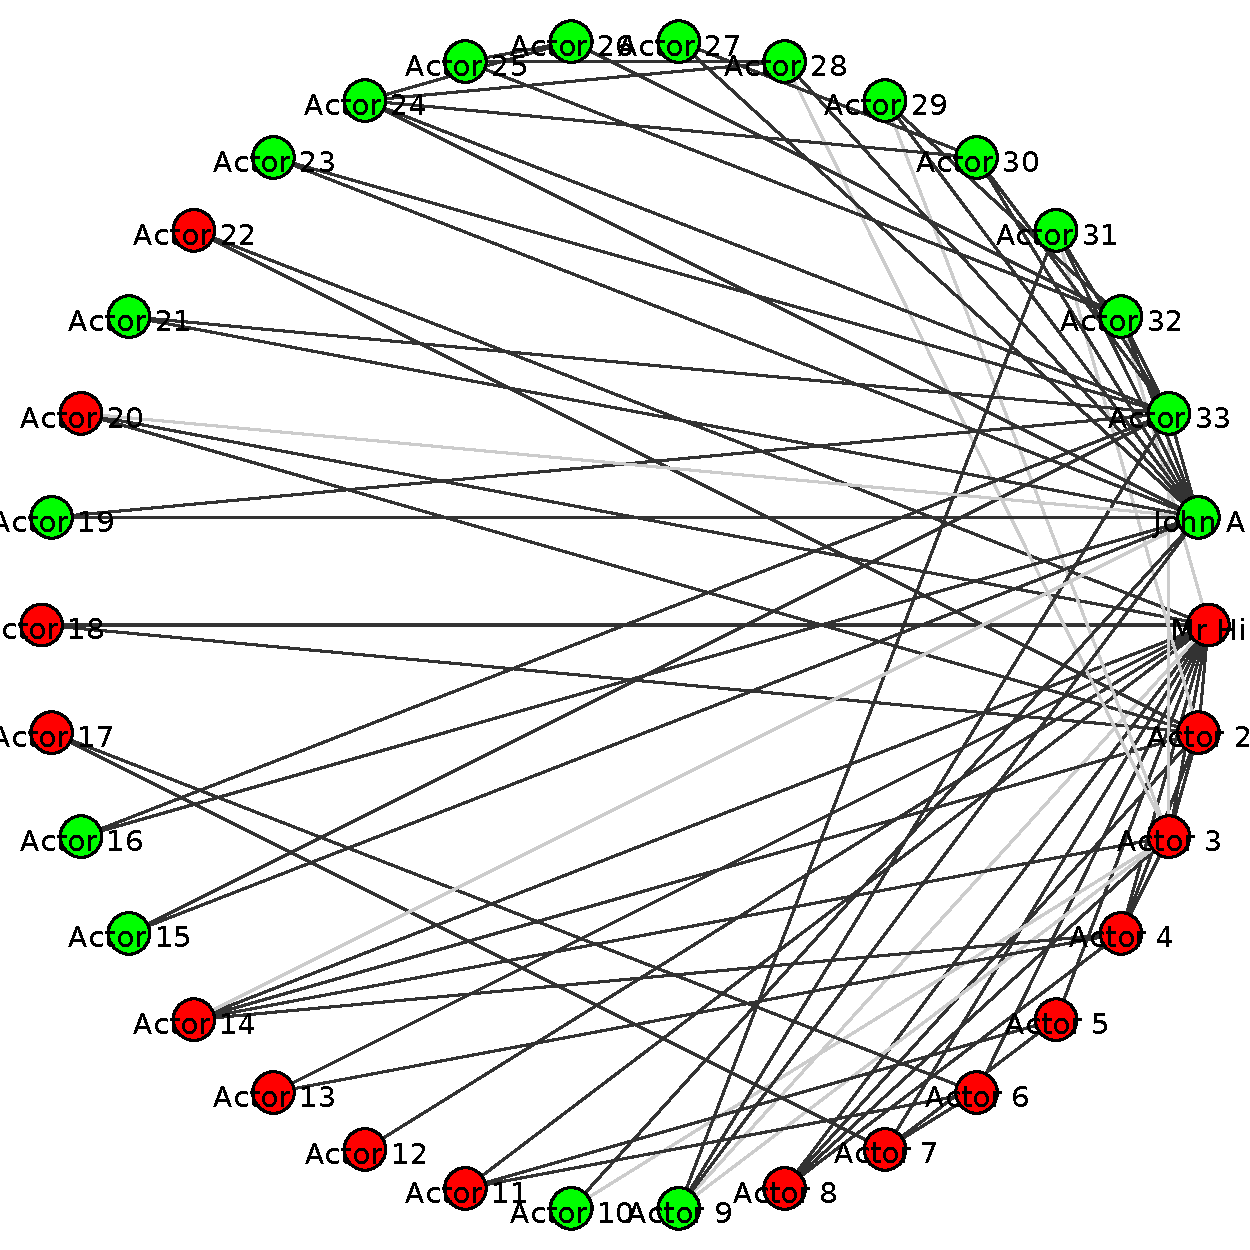
\includegraphics[width=2.5in]{eigenvector2.pdf}
  \captionof{figure}{Prediction of Leading Eigenvectors}
\end{minipage}
\end{figure}

As you can see, Newman's Leading Eigenvectors was able to correctly predict the split 100\%. 

Base on the results of the two algorithms, it is safe to say that the result of the karate club split could have been predicted by the weighted graph of social interactions. 

\lstinputlisting[language=python]{karate_club.py}

\section*{Problem 2}
We know the group split in two different groups. Suppose the
disagreements in the group were more nuanced -- what would the clubs
look like if they split into groups of 3, 4, and 5?

\subsection*{Answer}
To solve this problem, I just had to change the clusters number to get splits of 3 groups, 4 groups, and 5 groups. I did attempt to use Leading Eigenvectors algorithm at first, since it is more accurate. However, for this particular set of vertexes and relations, Leading Eigenvectors algorithms was not able to give sensible predictions after 3 splits. Therefore, I proceeded with Edgebetweenness algorithm. Also, to show the splits more clearly, I applied the Kamada-Kawai force-directed algorithm(kk) layout. 
\newpage

\begin{figure}[h]
\centering
\begin{minipage}{.5\textwidth}
  \centering
  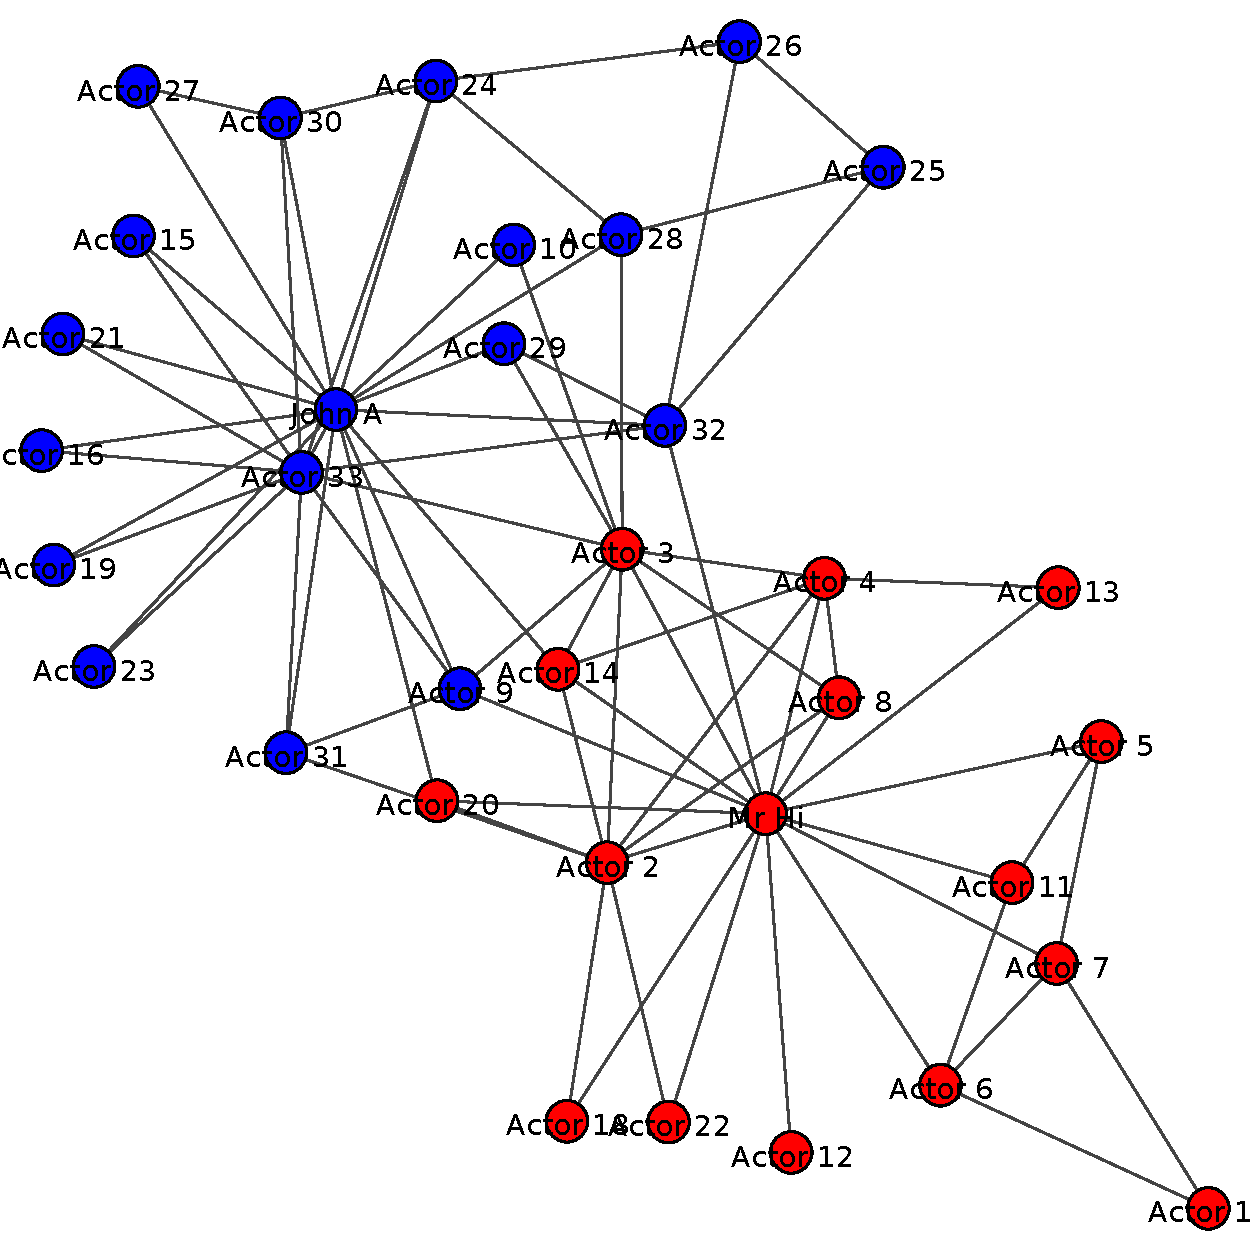
\includegraphics[width=2.5in]{aftersplitkk.pdf}
  \captionof{figure}{The actual split}
\end{minipage}%
\begin{minipage}{.5\textwidth}
  \centering
  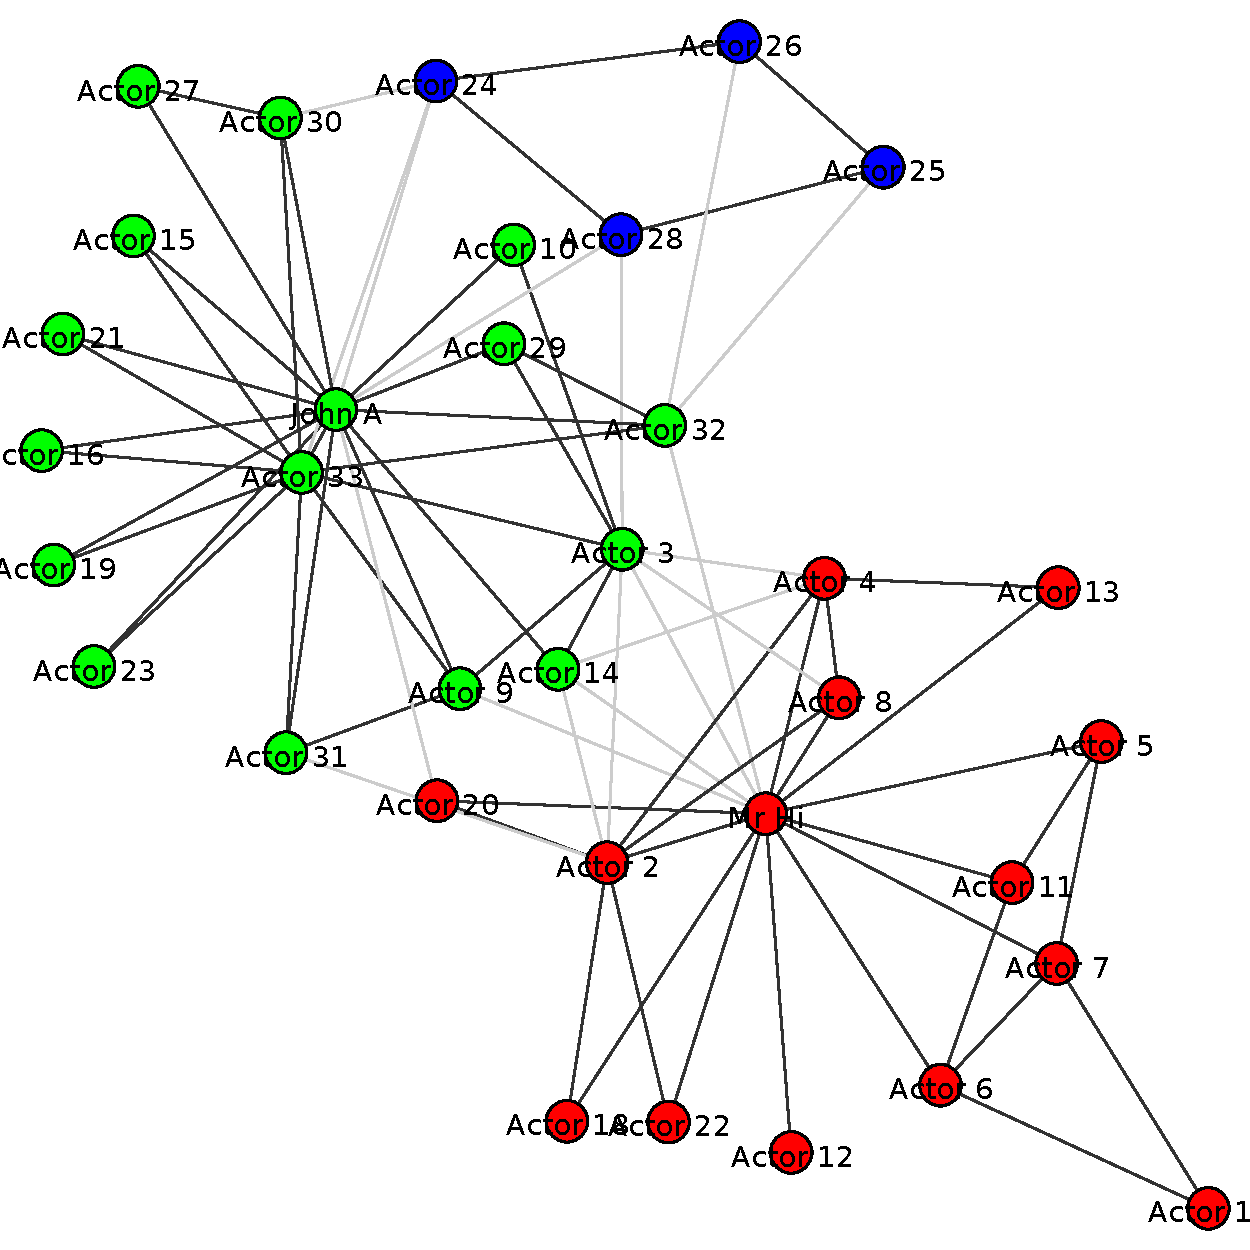
\includegraphics[width=2.5in]{betweenness3.pdf}
  \captionof{figure}{Club splits into 3 groups}
\end{minipage}
\end{figure}

\begin{figure}[h]
\centering
\begin{minipage}{.5\textwidth}
  \centering
  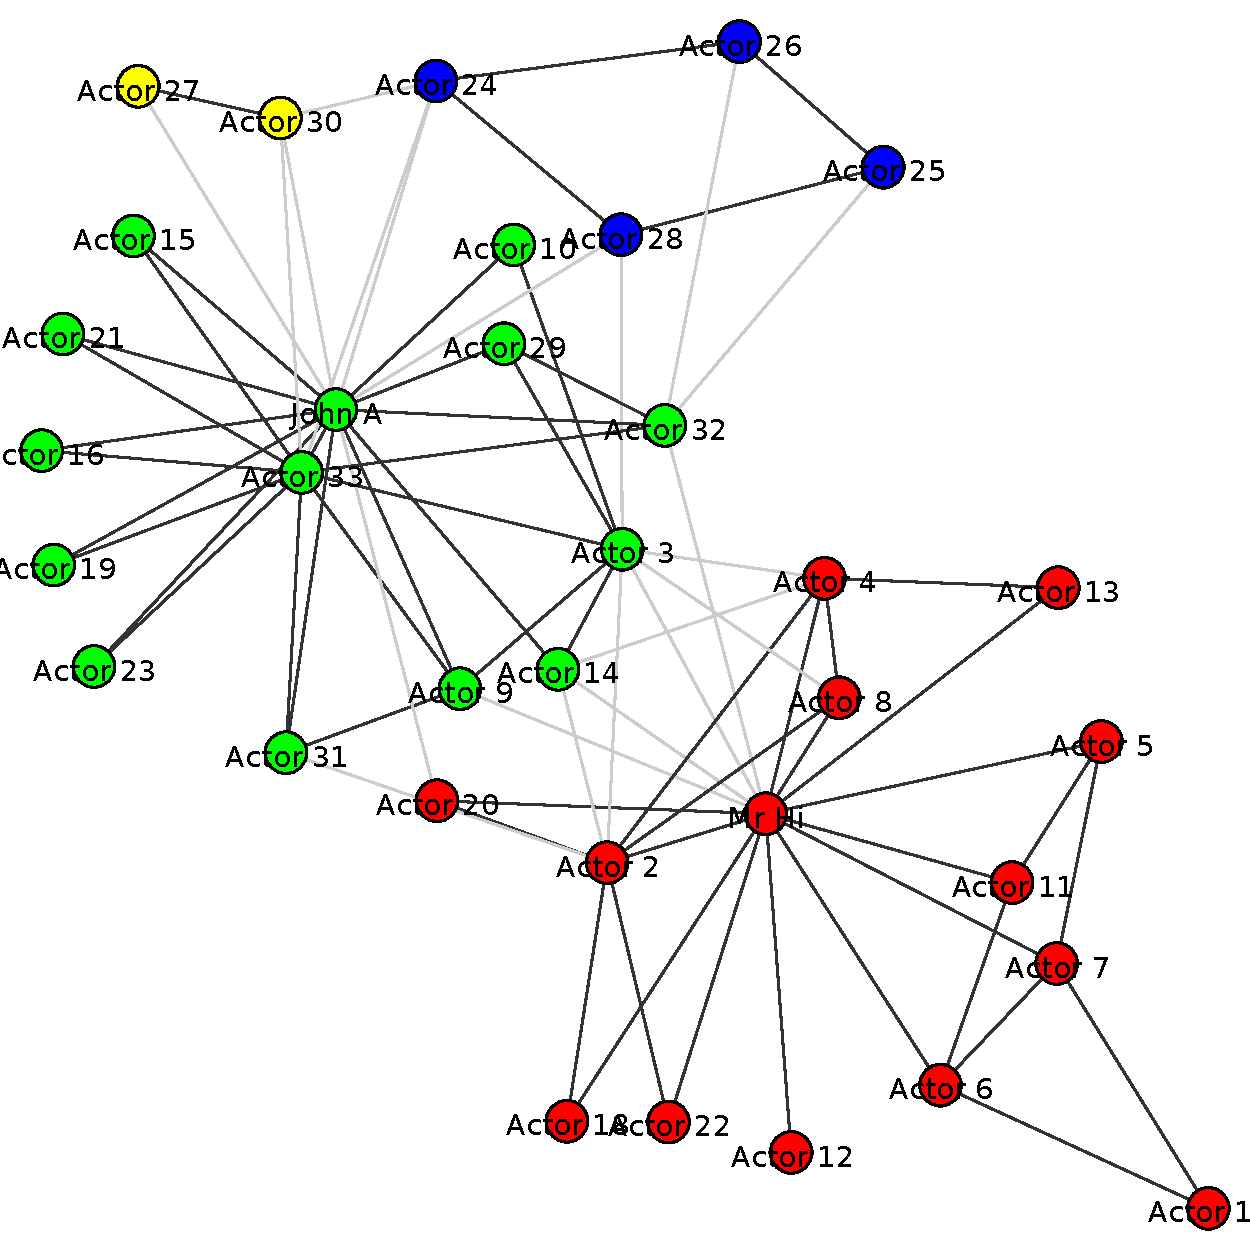
\includegraphics[width=2.5in]{betweenness4.pdf}
  \captionof{figure}{Club splits into 4 groups}
\end{minipage}%
\begin{minipage}{.5\textwidth}
  \centering
  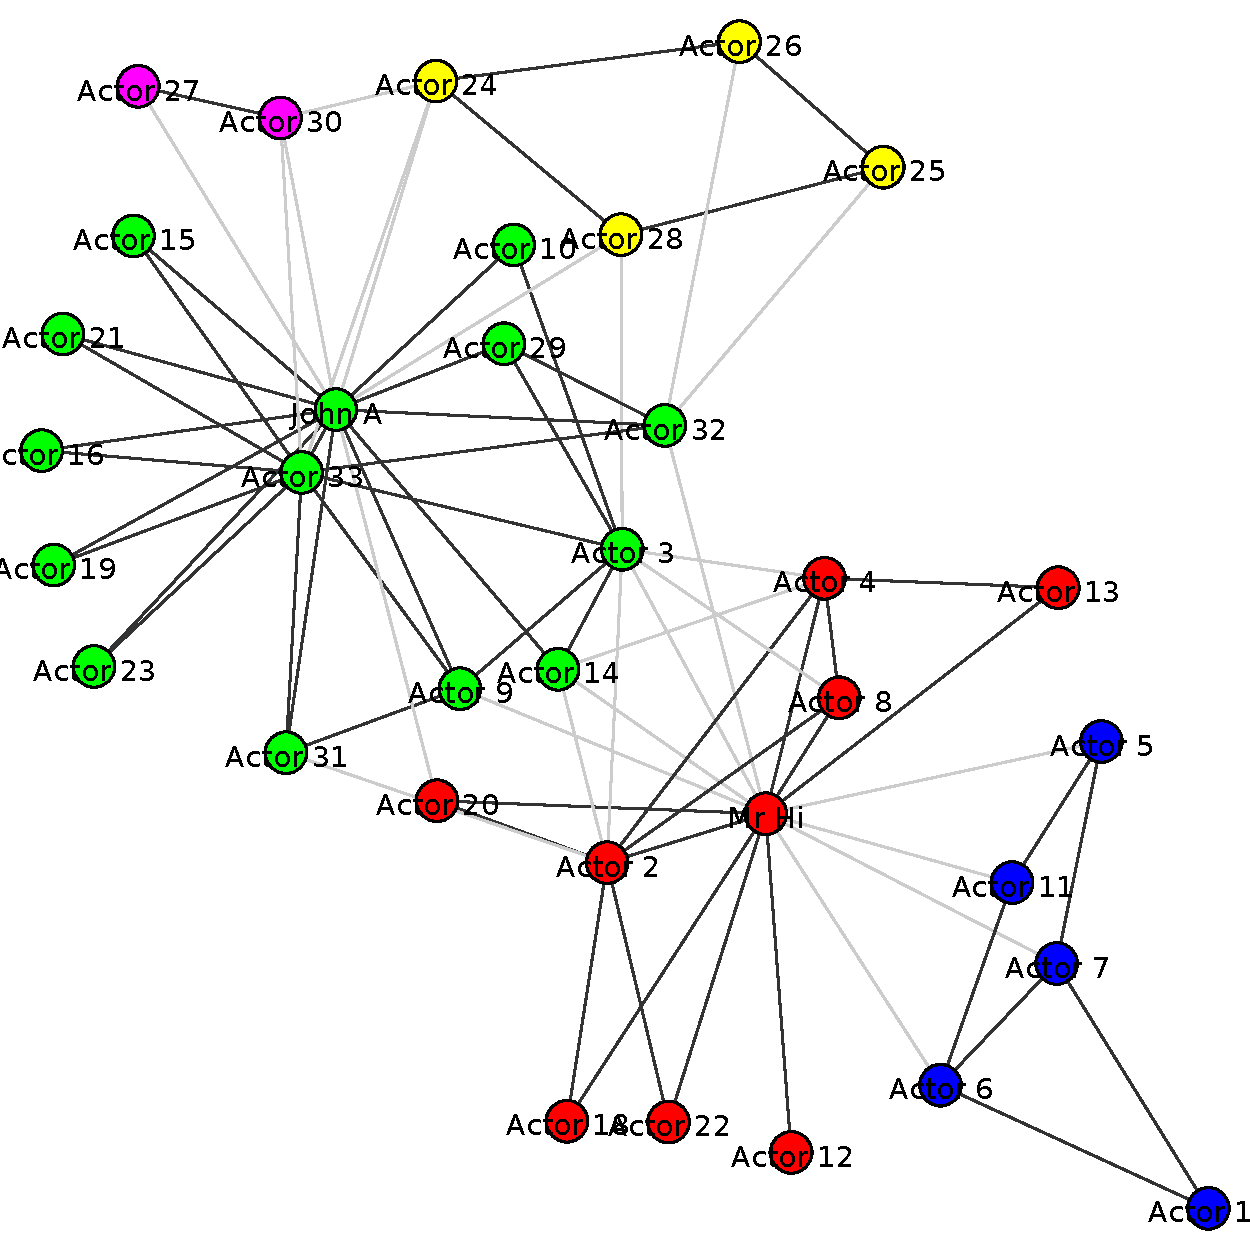
\includegraphics[width=2.5in]{betweenness5.pdf}
  \captionof{figure}{Club splits into 5 groups}
\end{minipage}
\end{figure}


\end{document}